\chapter{घूर्णी और कंपनिक स्पेक्ट्रमिकी}\label{ch:b3:rovibrational-spectroscopy}

एक ऊँचे, शुष्क पठार पर दर्जनों रेडियो एंटेना तारों के बीच एक अँधेरे मेघ की ओर
तने हैं। जो आवृत्तियाँ वे एकत्र करते हैं, उनमें एक
\qty{115.271}{GHz} पर है: कुछ केल्विन पर कार्बन मोनोऑक्साइड के अणु, जो अपने पहले
घूर्णी स्तर से निम्नतम स्तर पर आ रहे हैं। उसी एक संख्या से कोई
रसायनज्ञ C--O आबंध की लंबाई पिकोमीटर के एक अंश तक प्राप्त कर लेता है; अगली
रेखाओं की प्रबलताओं से मेघ का ताप। अणुओं के
घूर्णन और कंपन इस अध्याय का विषय हैं: उनके
स्तर, \cref{ch:b3:quantum-model-systems} के घूर्णक और दोलित्र से; वरण नियम,
\cref{ch:b3:group-theory-applied} से; और यह कि स्पेक्ट्रम क्या मापते हैं --- आबंध
लंबाइयाँ, \omterm{def:b3:quantum-model-systems:oscillator}{बल स्थिरांक}, वियोजन ऊर्जाएँ।

\begin{recall}
\Cref{ch:b3:quantum-model-systems} ने \omterm{def:b3:quantum-model-systems:rotor}{दृढ़ घूर्णक} दिया, $E_J = J(J+1)\hbar^2/2I$,
\omterm{def:b3:quantum-model-systems:degenerate}{अपभ्रष्टता} $2J + 1$ के साथ, और \omterm{def:b3:quantum-model-systems:oscillator}{आवर्ती दोलित्र}, $E_v = (v + \frac12)h\nu$,
\omterm{def:b3:quantum-model-systems:oscillator}{समानीत द्रव्यमान} $\mu$ वाले द्विपरमाणुक के लिए। \Cref{ch:b3:group-theory-applied} ने
अवरक्त और रामन वरण नियम बताए। प्रथम वर्ष के खंड ने अवरक्त
स्पेक्ट्रम तरंग-संख्याओं में मापे और अणु की ध्रुवणीयता परिभाषित की।
\end{recall}

\begin{omfigure}
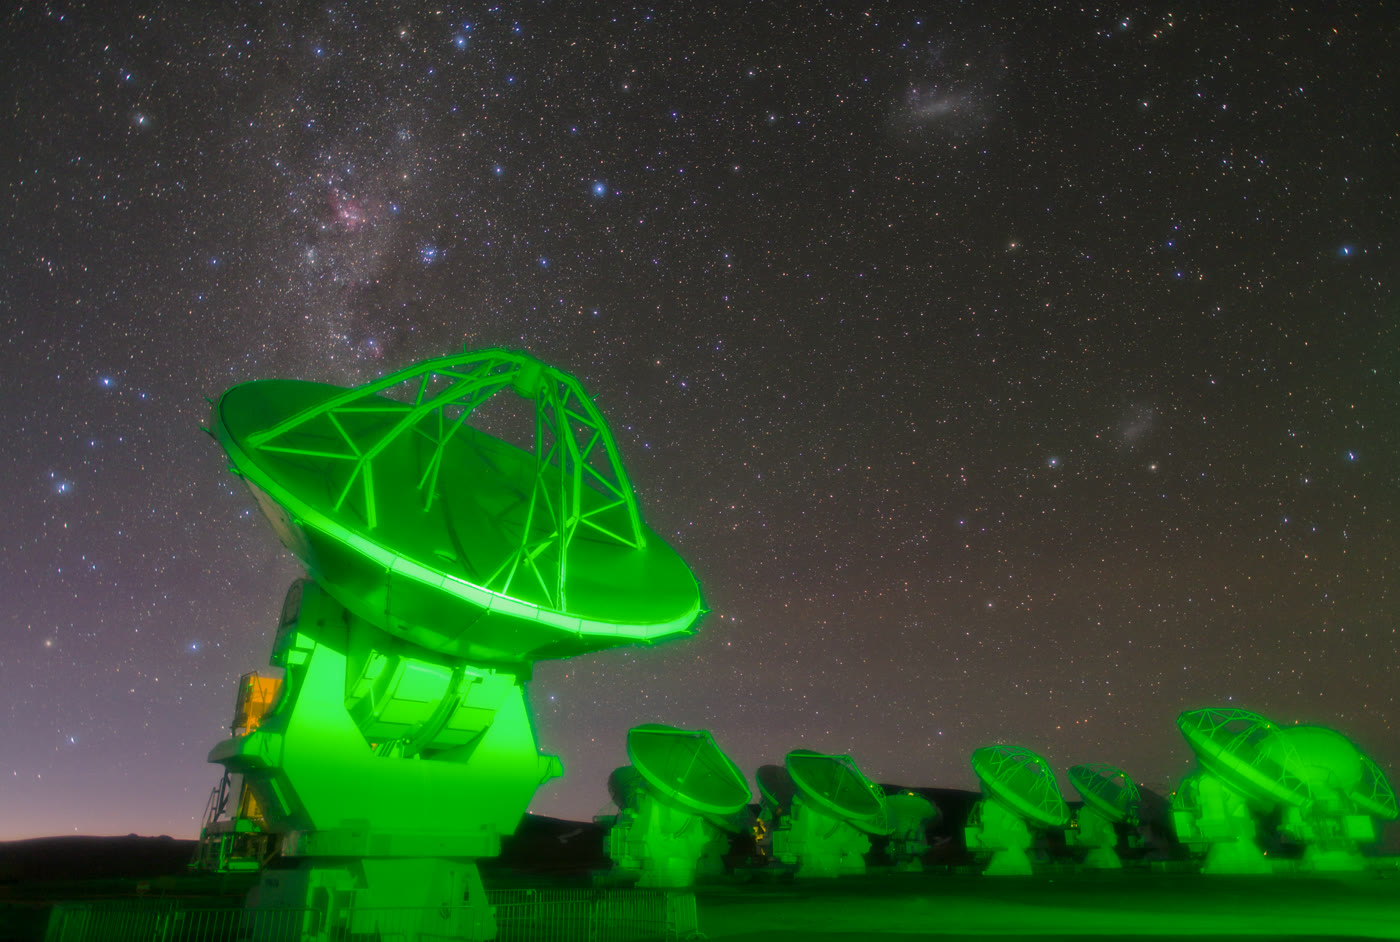
\includegraphics[width=0.7\linewidth]{images/book4/alma-antennas.jpg}

{\small एक ऊँचे पठार पर एक रेडियो व्यतिकरणमापी के एंटेना: वे अनेक
रेखाओं के साथ अंतरतारकीय मेघों से कार्बन मोनोऑक्साइड की घूर्णी रेखाएँ भी अभिलिखित करते हैं।
(छायाचित्र: ESO/बी॰~तफ़रेशी, \url{twanight.org}, CC BY 4.0।)}
\end{omfigure}

\section{घूर्णी स्पेक्ट्रम}

\begin{definition}[घूर्णन स्थिरांक, समस्थानिकरूपी]\label{def:b3:rovibrational-spectroscopy:rotational-constant}
रैखिक अणु का \emph{घूर्णन स्थिरांक}\index{घूर्णन स्थिरांक}
$B = h/(8\pi^2cI)$ है, \unit{cm^{-1}} में (या हर्ट्ज़ में $B = h/8\pi^2I$), ताकि उसके
घूर्णी स्तर तरंग-संख्याओं में $F(J) = BJ(J+1)$ हों। जो अणु केवल अपने परमाणुओं के
समस्थानिकों में भिन्न हैं, वे \emph{समस्थानिकरूपी}\index{समस्थानिकरूपी} हैं
(\ce{^{12}C^{16}O}, \ce{^{13}C^{16}O}); \omterm{def:b3:computational-chemistry:born-oppenheimer}{बॉर्न--ओपेनहाइमर सन्निकटन} में
उनकी आबंध लंबाइयाँ और \omterm{def:b3:quantum-model-systems:oscillator}{बल स्थिरांक} समान होते हैं।
\end{definition}

\begin{definition}[स्थूल और विशिष्ट वरण नियम]\label{def:b3:rovibrational-spectroscopy:selection}
\emph{स्थूल वरण नियम}\index{स्थूल वरण नियम} बताता है कि किसी अणु में
कौन-सा गुणधर्म होना चाहिए ताकि वह किसी प्रकार का स्पेक्ट्रम दिखा भी सके;
\emph{विशिष्ट वरण नियम}\index{विशिष्ट वरण नियम} बताता है कि क्वांटम संख्या के
कौन-से परिवर्तन अनुमत हैं।
\end{definition}

\begin{proposition}[शुद्ध घूर्णी स्पेक्ट्रम]\label{prop:b3:rovibrational-spectroscopy:rotational-lines}
किसी अणु का शुद्ध घूर्णी (सूक्ष्मतरंग) स्पेक्ट्रम केवल तभी होता है जब उसका
स्थायी द्विध्रुव आघूर्ण हो; रैखिक अणु के लिए विशिष्ट नियम $\Delta J
= \pm1$ है। अवशोषण रेखाएँ इन पर होती हैं:
\[
\tilde\nu = F(J+1) - F(J) = 2B(J + 1), \qquad J = 0, 1, 2, \dots,
\]
जो $2B$ के समान अंतरालों पर हैं।
\end{proposition}

\begin{proof}
प्रकाश के साथ अन्योन्यक्रिया द्विध्रुव आघूर्ण के माध्यम से होती है: जिस अणु का कोई
स्थायी द्विध्रुव नहीं है, घूमने पर उसका कोई दोलायमान द्विध्रुव नहीं होता। नियम $\Delta J
= \pm1$, $\int Y_{J'M'}^*\cos\theta\,Y_{JM}$ के लुप्त होने से आता है, जब तक कि $J' = J
\pm 1$ न हो ($z$ के अनुदिश द्विध्रुव घटक $Y_{1,0}$ की तरह रूपांतरित होता है), स्वीकृत।
तब $B(J+1)(J+2) - BJ(J+1) = 2B(J+1)$।
\end{proof}

\begin{method}[घूर्णी रेखा से आबंध लंबाई]\label{met:b3:rovibrational-spectroscopy:bond-length}
\begin{enumerate}
  \item रेखा $J + 1 \leftarrow J$ से, जो आवृत्ति $\nu$ पर है, $B =
        \nu/2(J+1)$ निकालिए (हर्ट्ज़ में)।
  \item जड़त्व आघूर्ण $I = h/8\pi^2B$ परिकलित कीजिए।
  \item समस्थानिक द्रव्यमानों से प्राप्त \omterm{def:b3:quantum-model-systems:oscillator}{समानीत द्रव्यमान} के साथ, $r = \sqrt{I/\mu}$।
\end{enumerate}
\end{method}

\begin{example}[कार्बन मोनोऑक्साइड]\label{ex:b3:rovibrational-spectroscopy:co}\emergencystretch=3em
% ledger: rotl:CO.1-0, imass:O16
\ce{^{12}C^{16}O} की रेखा $J = 1 \leftarrow 0$, \qty{115271.20}{MHz} पर है:
$B = \qty{57635.6}{MHz} = \qty{1.92252}{cm^{-1}}$, $I = \qty{1.4560e-46}{kg.m^2}$।
$\mu = 12 \times 15.99491/27.99491 = \qty{6.85621}{u}$ के साथ $r_0 = \qty{113.09}{pm}$।
यह $r_0$ आबंध का उसके शून्य-बिंदु कंपन पर औसत है और साम्य लंबाई $r_e$ से
थोड़ा लंबा है (\cref{sec:b3:rovibrational-spectroscopy:real-bonds})।
\end{example}

\begin{definition}[अपकेंद्री विरूपण स्थिरांक]\label{def:b3:rovibrational-spectroscopy:centrifugal}
घूमता हुआ आबंध खिंच जाता है; स्तर $F(J) = BJ(J+1) - DJ^2(J+1)^2$ हो जाते हैं,
जहाँ $D$ \emph{अपकेंद्री विरूपण स्थिरांक}\index{अपकेंद्री विरूपण स्थिरांक} है,
और रेखाएँ $2B(J+1) - 4D(J+1)^3$ ऊँचे $J$ पर धीरे-धीरे पास आती
जाती हैं।
\end{definition}

\begin{proposition}[सबसे प्रबल रेखा]\label{prop:b3:rovibrational-spectroscopy:jmax}
यदि रेखाओं की तीव्रताएँ निचले स्तर की समष्टि, $(2J+1)
\eu^{-hcBJ(J+1)/kT}$, का अनुसरण करती हैं, तो सबसे अधिक समष्टित स्तर इसके निकट है:
\[
J_{\max} \approx \sqrt{\frac{kT}{2hcB}} - \frac12.
\]
\end{proposition}

\begin{proof}
$J$ को संतत मानकर अवकलन कीजिए: $\frac{\dd}{\dd J}[(2J+1)\eu^{-aJ(J+1)}]
= [2 - a(2J+1)^2]\eu^{-aJ(J+1)}$, जहाँ $a = hcB/kT$; यह $(2J + 1)^2 =
2/a$ पर लुप्त होता है।
\end{proof}

\begin{omfigure}
\begin{tikzpicture}
\begin{axis}[width=0.9\linewidth, height=4.8cm, xmin=0, xmax=70, ymin=0,
  ymax=1.12, ytick=\empty, axis x line=bottom, axis y line=left, ycomb,
  xlabel={तरंग-संख्या / cm$^{-1}$}, ylabel={आपेक्षिक तीव्रता},
  tick label style={font=\small}, label style={font=\small}]
\addplot[omDef, very thick] table[x=nu, y=I] {figdata/out/bachelor-3-rotational-spectrum-co-30.dat};
\addplot[omThm, thick, xshift=1.2pt] table[x=nu, y=I] {figdata/out/bachelor-3-rotational-spectrum-co-300.dat};
\end{axis}
\end{tikzpicture}

{\small कार्बन मोनोऑक्साइड का घूर्णी अवशोषण स्पेक्ट्रम, रेखाओं के बीच
$2B = \qty{3.845}{cm^{-1}}$ का अंतराल, तीव्रताएँ निचले स्तर की समष्टि के रूप में ली गई हैं,
\qty{30}{K} (नीला) और \qty{300}{K} (लाल, दृश्यता के लिए थोड़ा
खिसकाया गया) पर, हर ताप अपनी सबसे प्रबल रेखा के सापेक्ष मापित। \qty{30}{K} पर सबसे प्रबल रेखा
$J = 3 \leftarrow 2$ है; \qty{300}{K} पर $J = 8 \leftarrow 7$।}
\end{omfigure}

\section{वास्तविक आबंधों के कंपन}\label{sec:b3:rovibrational-spectroscopy:real-bonds}

वास्तविक आबंध साम्य से दूर हुक के नियम का पालन नहीं करता: खींचने पर वह नरम
पड़ता है और टूट जाता है।

\begin{definition}[मोर्स विभव]\label{def:b3:rovibrational-spectroscopy:morse}
\emph{मोर्स विभव}\index{मोर्स विभव} $V(r) = D_e[1 -
\eu^{-\beta(r - r_e)}]^2$ है: $r_e$ के निकट आवर्ती (\omterm{def:b3:quantum-model-systems:oscillator}{बल स्थिरांक} $2\beta^2D_e$), और
वियोजन सीमा $D_e$ की ओर प्रवृत्त, बड़े $r$ पर।
\end{definition}

\begin{proposition}[मोर्स दोलित्र के स्तर]\label{prop:b3:rovibrational-spectroscopy:morse-levels}
तरंग-संख्याओं में मोर्स दोलित्र के कंपनिक स्तर ये हैं:
\[
G(v) = \tilde\omega_e(v + \tfrac12) - \tilde\omega_ex_e(v + \tfrac12)^2, \qquad
\tilde\omega_ex_e = \frac{\tilde\omega_e^2}{4D_e},
\]
एक सीढ़ी जिसके डंडे पास आते जाते हैं और $v_{\max} = \lfloor\tilde\omega_e/
2\tilde\omega_ex_e - \frac12\rfloor$ पर समाप्त होते हैं।
\end{proposition}
\admitted

मोर्स समीकरण का हल अधिक उन्नत पाठ्यक्रमों में दिया जाता है;
स्तरों की संख्यात्मक जाँच इस अध्याय के चित्र-आँकड़ों में की गई है।

\begin{definition}[अनावर्तिता स्थिरांक, मूल संक्रमण, अधिस्वरक, तप्त बैंड]\label{def:b3:rovibrational-spectroscopy:anharmonic}
$\tilde\omega_ex_e$ \emph{अनावर्तिता स्थिरांक}\index{अनावर्तिता स्थिरांक} है।
\emph{मूल संक्रमण}\index{मूल संक्रमण}
$v = 1 \leftarrow 0$ है; \emph{अधिस्वरक}\index{अधिस्वरक} $v = n \leftarrow 0$ है,
जहाँ $n \ge 2$, जो दुर्बल होता है क्योंकि \omterm{def:b3:quantum-model-systems:oscillator}{आवर्ती दोलित्र} का स्थूल नियम $\Delta v = \pm1$
केवल थोड़ा-सा टूटता है; \emph{तप्त बैंड}\index{तप्त बैंड} किसी उत्तेजित स्तर से
आरंभ होता है, $v = 2 \leftarrow 1$, और ताप के साथ बढ़ता है।
\end{definition}

\begin{definition}[स्पेक्ट्रमी वियोजन ऊर्जा]\label{def:b3:rovibrational-spectroscopy:dissociation}
किसी अणु की \emph{स्पेक्ट्रमी वियोजन ऊर्जा}\index{स्पेक्ट्रमी वियोजन ऊर्जा}
उसके विभव की गहराई $D_e$ है, जो निम्निष्ठ से मापी जाती है,
या $D_0 = D_e - G(0)$, जो निम्नतम स्तर से मापी जाती है --- प्रति
अणु, \qty{0}{K} पर, द्वितीय वर्ष के खंड की आबंध वियोजन एन्थैल्पी के विपरीत,
जो \qty{298}{K} पर एक मोलर एन्थैल्पी है।
\end{definition}

\begin{corollary}[मोर्स दोलित्र के $D_e$ और $D_0$]\label{cor:b3:rovibrational-spectroscopy:de}
$D_e = \tilde\omega_e^2/4\tilde\omega_ex_e$ और $D_0 = D_e - (\frac12\tilde\omega_e -
\frac14\tilde\omega_ex_e)$।
\end{corollary}

\begin{proof}
पहला प्रतिज्ञप्ति का संबंध है; दूसरा $G(0)$ है।
\end{proof}

\begin{proposition}[बर्ज--स्पोनर बहिर्वेशन]\label{prop:b3:rovibrational-spectroscopy:birge-sponer}
अंतराल $\Delta G(v + \frac12) = G(v+1) - G(v) = \tilde\omega_e - 2\tilde\omega_ex_e(v +
1)$, $v$ के साथ रैखिक रूप से घटते हैं; उनके लुप्त होने तक उनका योग $D_0$ देता है,
अर्थात् $\Delta G$ को $v$ के विरुद्ध आलेखित करने पर आलेख के नीचे का क्षेत्रफल।
\end{proposition}

\begin{proof}
$G$ के दोनों व्यंजकों को घटाइए। $D_0$, $v = 0$ से
सीमा तक की ऊर्जा है, सभी अंतरालों का योग।
\end{proof}

\begin{example}[हाइड्रोजन क्लोराइड]\label{ex:b3:rovibrational-spectroscopy:hcl}
% ledger: diat:HCl.we, diat:HCl.wexe, janaf:H.dfH0, janaf:Cl.dfH0, janaf:HCl.dfH0
\ce{H^{35}Cl} के लिए $\tilde\omega_e = \qty{2990.95}{cm^{-1}}$ और $\tilde\omega_ex_e =
\qty{52.82}{cm^{-1}}$: \omterm{def:b3:rovibrational-spectroscopy:anharmonic}{मूल संक्रमण} $\tilde\omega_e - 2\tilde\omega_ex_e =
\qty{2885.3}{cm^{-1}}$ पर है और पहला \omterm{def:b3:rovibrational-spectroscopy:anharmonic}{अधिस्वरक} $2\tilde\omega_e - 6\tilde\omega_ex_e =
\qty{5665.0}{cm^{-1}}$ पर, \omterm{def:b3:rovibrational-spectroscopy:anharmonic}{मूल संक्रमण} के दुगुने से थोड़ा कम। मोर्स मॉडल
$D_e = \qty{42342}{cm^{-1}}$ और $D_0 = \qty{40860}{cm^{-1}}$ बताता है; वास्तविक $D_0$,
\qty{0}{K} पर H, Cl और HCl की संभवन एन्थैल्पियों से,
\qty{35760}{cm^{-1}} (\qty{4.43}{eV}) है। वास्तविक विभव तली पर समंजित मोर्स वक्र
की तुलना में जल्दी सपाट हो जाता है: निम्नतम स्तरों से किए गए बर्ज--स्पोनर
बहिर्वेशन वियोजन ऊर्जाओं को अधिक आँकते हैं।
\end{example}

\begin{omfigure}
\begin{tikzpicture}
\begin{axis}[name=morse, width=0.55\linewidth, height=6cm, xmin=0.8, xmax=4.0,
  ymin=0, ymax=48000, axis lines=left, xlabel={$r$ / \AA}, ylabel={$V$ / cm$^{-1}$},
  unbounded coords=jump, scaled y ticks=false, ytick={0,10000,20000,30000,40000},
  tick label style={font=\small}, label style={font=\small}]
\addplot[black, thick] table[x=r, y=V] {figdata/out/bachelor-3-morse-levels.dat};
\addplot[gray, dashed] table[x=r, y=harm] {figdata/out/bachelor-3-morse-levels.dat};
\addplot[omDef] table[x=r, y=E] {figdata/out/bachelor-3-morse-levels-levels.dat};
\draw[<->, omThm] (axis cs:3.7,0) -- (axis cs:3.7,42342) node[pos=0.5, left, font=\small] {$D_e$};
\draw[dashed, omThm] (axis cs:1.2,42342) -- (axis cs:4.0,42342);
\end{axis}
\begin{axis}[at={(morse.east)}, anchor=west, xshift=1.6cm, width=0.4\linewidth,
  height=5cm, xmin=0, xmax=28, ymin=0, ymax=3100, axis lines=left,
  xlabel={$v$}, ylabel={$\Delta G(v + \frac12)$ / cm$^{-1}$},
  tick label style={font=\small}, label style={font=\small}]
\addplot[omDef, only marks, mark size=1.2pt] table[x=v, y=dG] {figdata/out/bachelor-3-morse-levels-bs.dat};
\addplot[omDef!40, fill=omDef!12, draw=none] table[x=v, y=dG] {figdata/out/bachelor-3-morse-levels-bs.dat} \closedcycle;
\end{axis}
\end{tikzpicture}

{\small बाएँ: \ce{HCl} का \omterm{def:b3:rovibrational-spectroscopy:morse}{मोर्स विभव}, उसके स्पेक्ट्रमी स्थिरांकों से
बना (सतत रेखा), समान वक्रता वाला आवर्ती परवलय (खंडित),
और हर तीसरा कंपनिक स्तर, जो अपने व्यावर्तन बिंदुओं के बीच खींचा गया है;
स्तर $D_e$ की ओर पास आते जाते हैं। दाएँ: अंतरालों का बर्ज--स्पोनर आलेख;
छायांकित क्षेत्रफल $D_0$ है।}
\end{omfigure}

\section{घूर्णी-कंपनिक बैंड}

किसी गैस का कंपनिक संक्रमण घूर्णी परिवर्तनों के साथ होता है, $\Delta
J = \pm1$, ${}^1\Sigma$ अवस्था वाले द्विपरमाणुक के लिए।

\begin{definition}[P, Q और R शाखाएँ, बैंड मूल]\label{def:b3:rovibrational-spectroscopy:branches}
घूर्णी-कंपनिक बैंड में $\Delta J = -1$ वाली रेखाएँ \emph{P
शाखा}\index{P शाखा} बनाती हैं, $\Delta J = +1$ वाली \emph{R शाखा}\index{R शाखा},
और $\Delta J = 0$ वाली, जब अनुमत हों, \emph{Q शाखा}\index{Q शाखा}।
\emph{बैंड मूल}\index{बैंड मूल} $\tilde\nu_0$ घूर्णन के बिना
कंपनिक ऊर्जा-अंतर है।
\end{definition}

\begin{theorem}[संयोजन अंतर]\label{thm:b3:rovibrational-spectroscopy:combination-differences}
निचले और ऊपरी कंपनिक स्तरों में \omterm{def:b3:rovibrational-spectroscopy:rotational-constant}{घूर्णन स्थिरांक} $B_0$ और $B_1$ के साथ,
$R(J) = \tilde\nu_0 + B_1(J+1)(J+2) - B_0J(J+1)$ और $P(J) = \tilde\nu_0 +
B_1(J-1)J - B_0J(J+1)$, और
\[
R(J - 1) - P(J + 1) = 4B_0(J + \tfrac12), \qquad R(J) - P(J) = 4B_1(J + \tfrac12).
\]
\end{theorem}

\begin{proof}
पहले दो, दोनों स्तरों के लिए $E = G(v) + B_vJ(J+1)$ से निकलते हैं। $R(J - 1)$ और
$P(J + 1)$ एक ही ऊपरी स्तर $J$ पर समाप्त होते हैं, निचले स्तरों $J - 1$ और $J + 1$ से:
उनका अंतर $B_0[(J+1)(J+2) - (J-1)J] = B_0(4J + 2)$ है। इसी प्रकार $R(J)$ और
$P(J)$ एक ही निचले स्तर से आरंभ होते हैं और $J + 1$ तथा $J - 1$ पर समाप्त होते हैं।
\end{proof}

\begin{method}[घूर्णी-कंपनिक बैंड का विश्लेषण]\label{met:b3:rovibrational-spectroscopy:combination}
\begin{enumerate}
  \item रिक्ति ढूँढ़िए: ${}^1\Sigma$ द्विपरमाणुक के लिए कोई \omterm{def:b3:rovibrational-spectroscopy:branches}{Q शाखा} नहीं होती, और
        $\tilde\nu_0$ रिक्ति में, $R(0)$ और $P(1)$ के बीच, होता है।
  \item रिक्ति से बाहर की ओर रेखाओं को क्रमांकित कीजिए: $R(0), R(1), \dots$ और $P(1),
        P(2), \dots$।
  \item संयोजन अंतरों से $B_0$ और $B_1$
        अलग-अलग प्राप्त कीजिए, फिर $\alpha_e = B_0 - B_1$ और $B_e = B_0 + \frac12\alpha_e$।
\end{enumerate}
\end{method}

\begin{omfigure}
\begin{tikzpicture}
\begin{axis}[width=0.92\linewidth, height=5cm, xmin=2650, xmax=3080, ymin=0,
  ymax=1.15, ytick=\empty, axis x line=bottom, axis y line=left,
  xlabel={तरंग-संख्या / cm$^{-1}$}, ylabel={अवशोषकता (आपेक्षिक)},
  tick label style={font=\small}, label style={font=\small}]
\addplot[omDef, thin] table[x=nu, y=A] {figdata/out/bachelor-3-rovib-band.dat};
\node[font=\small] at (axis cs:2780,1.06) {P शाखा};
\node[font=\small] at (axis cs:2985,1.06) {R शाखा};
\draw[->, gray] (axis cs:2885.3,0.45) -- (axis cs:2885.3,0.05);
\node[font=\small, gray, anchor=south] at (axis cs:2885.3,0.45) {$\tilde\nu_0$};
\end{axis}
\end{tikzpicture}

{\small \qty{300}{K} पर गैसीय \ce{HCl} का मूल बैंड, उसके स्पेक्ट्रमी स्थिरांकों से
परिकलित: \omterm{def:b3:rovibrational-spectroscopy:branches}{बैंड मूल} पर स्थित रिक्ति के दोनों ओर P और \omterm{def:b3:rovibrational-spectroscopy:branches}{R शाखाएँ}। हर रेखा एक द्विक है,
\ce{H^{35}Cl} और उससे दुर्बल, थोड़ी नीचे स्थित
\ce{H^{37}Cl} (प्राकृतिक प्रचुरताएँ 76\,\% और 24\,\%)। R रेखाएँ पास आती जाती हैं,
P रेखाएँ फैलती जाती हैं, क्योंकि $B_1 < B_0$।}
\end{omfigure}

\begin{example}[बैंड से \ce{HCl} के स्थिरांक]\label{ex:b3:rovibrational-spectroscopy:analysis}\emergencystretch=3em
% ledger: diat:HCl.Be, diat:HCl.ae
$R(0) = \qty{2905.58}{cm^{-1}}$ और $P(2) = \qty{2842.94}{cm^{-1}}$ से
$6B_0 = \qty{62.64}{cm^{-1}}$ मिलता है, अतः $B_0 = \qty{10.440}{cm^{-1}}$। $R(1) = 2925.23$ और $P(1) =
\qty{2864.43}{cm^{-1}}$ से $B_1 = \qty{10.133}{cm^{-1}}$। अतः $\alpha_e = \qty{0.307}{cm^{-1}}$
और $B_e = \qty{10.593}{cm^{-1}}$, वही मान जिनसे बैंड बनाया गया था:
विधि उन्हें यथार्थतः पुनः प्राप्त कर लेती है।
\end{example}

\section{रामन स्पेक्ट्रमिकी}

\begin{definition}[रामन और रैले प्रकीर्णन]\label{def:b3:rovibrational-spectroscopy:raman}
जब आवृत्ति $\nu_0$ का प्रकाश किसी नमूने को पार करता है, तो अधिकांश प्रकीर्णित प्रकाश
आवृत्ति $\nu_0$ बनाए रखता है: यह \emph{रैले प्रकीर्णन}\index{रैले प्रकीर्णन} है।
एक छोटा अंश अणुओं की घूर्णी या कंपनिक आवृत्तियों जितना
विस्थापित हो जाता है: यह \emph{रामन प्रकीर्णन}\index{रामन प्रकीर्णन} है।
निम्नतर आवृत्ति की रेखाएँ \emph{स्टोक्स रेखाएँ}\index{स्टोक्स रेखा} हैं (अणु ने
ऊर्जा प्राप्त की), उच्चतर आवृत्ति की \emph{प्रति-स्टोक्स
रेखाएँ}\index{प्रति-स्टोक्स रेखा} (उसने ऊर्जा खोई)।
\end{definition}

\begin{proposition}[रामन प्रभाव का चिरसम्मत मूल]\label{prop:b3:rovibrational-spectroscopy:raman-classical}
यदि $\nu_{\mathrm{vib}}$ पर कंपन करते अणु की ध्रुवणीयता
$\alpha = \alpha_0 + \alpha_1\cos(2\pi\nu_{\mathrm{vib}}t)$ के रूप में बदलती है, तो
क्षेत्र $E_0\cos(2\pi\nu_0t)$ द्वारा प्रेरित द्विध्रुव $\nu_0$ पर और $\nu_0 \pm \nu_{\mathrm{vib}}$ पर दोलन करता है।
कोई कंपन केवल तभी \omterm{def:b3:group-theory-applied:activity}{रामन-सक्रिय} है जब वह ध्रुवणीयता को बदले।
\end{proposition}

\begin{proof}
$\mu = \alpha E = \alpha_0E_0\cos(2\pi\nu_0t) + \frac12\alpha_1E_0[\cos2\pi(\nu_0 +
\nu_{\mathrm{vib}})t + \cos2\pi(\nu_0 - \nu_{\mathrm{vib}})t]$, $\cos a\cos b =
\frac12[\cos(a+b) + \cos(a-b)]$ से। हर दोलायमान द्विध्रुव अपनी ही
आवृत्ति पर विकिरण करता है; $\alpha_1$ के बिना केवल रैले पद बचता है।
\end{proof}

\begin{proposition}[घूर्णी रामन रेखाएँ]\label{prop:b3:rovibrational-spectroscopy:rotational-raman}
विषमदैशिक ध्रुवणीयता वाला रैखिक अणु $\Delta J = \pm2$ वाली घूर्णी रामन
रेखाएँ दिखाता है, जो उत्तेजक रेखा से इतनी विस्थापित होती हैं:
\[
|\Delta\tilde\nu| = F(J+2) - F(J) = 4B(J + \tfrac32) = 6B, 10B, 14B, \dots
\]
--- पहली रेखा $6B$ पर, फिर $4B$ का अंतराल।
\end{proposition}

\begin{proof}
घूमते रैखिक अणु का ध्रुवणीयता दीर्घवृत्तज प्रति घूर्णन दो बार उसी
अभिविन्यास में लौटता है, अतः वह प्रकीर्णन को घूर्णन आवृत्ति की दुगुनी आवृत्ति पर
मॉडुलित करता है: $\Delta J = \pm2$ (क्वांटम नियम, स्वीकृत)। तब
$B(J+2)(J+3) - BJ(J+1) = B(4J + 6)$।
\end{proof}

\begin{example}[रामन द्वारा देखा गया नाइट्रोजन]\label{ex:b3:rovibrational-spectroscopy:n2}
% ledger: diat:N2.Be, diat:N2.ae
\ce{N2} का कोई द्विध्रुव नहीं है और कोई अवरक्त या सूक्ष्मतरंग स्पेक्ट्रम नहीं, परंतु उसकी
ध्रुवणीयता विषमदैशिक है: उसकी घूर्णी रामन रेखाएँ उत्तेजक रेखा से $6B_0 =
\qty{11.94}{cm^{-1}}$ पर आरंभ होती हैं और उनके बीच \qty{7.96}{cm^{-1}} का अंतराल है। उनकी
तीव्रताएँ सम और विषम $J$ के बीच 2:1 के अनुपात में एकांतरित होती हैं: दोनों \ce{^{14}N} नाभिक
सर्वसम हैं, और नाभिकीय-चक्रण सांख्यिकी (\cref{ch:b3:statistical-thermo-applied})
सम-$J$ स्तरों को विषम स्तरों से दुगुना भार देती है।
\end{example}

\begin{omfigure}
\begin{tikzpicture}
\begin{axis}[name=r, width=0.55\linewidth, height=4.6cm, xmin=-110, xmax=110,
  ymin=0, ymax=1.1, ytick=\empty, axis x line=bottom, axis y line=left, ycomb,
  xlabel={रामन विस्थापन / cm$^{-1}$}, tick label style={font=\small}, label style={font=\small},
  title={\small \ce{N2}, घूर्णी रामन, \qty{300}{K}}]
\addplot[omDef, thick] table[x=shift, y=I] {figdata/out/bachelor-3-rotational-spectrum-n2-raman.dat};
\draw[gray, thick] (axis cs:0,0) -- (axis cs:0,1.05);
\end{axis}
\begin{scope}[xshift=0.6\linewidth, font=\small]
  \draw[omstate] (0,0) -- (2.4,0) node[right] {$v = 0$};
  \draw[omstate] (0,1.0) -- (2.4,1.0) node[right] {$v = 1$};
  \draw[omvib, densely dashed] (0,3.2) -- (2.4,3.2) node[right] {आभासी};
  \draw[omabs] (0.3,0) -- (0.3,3.18);
  \draw[omfluo] (0.5,3.18) -- (0.5,0.02);
  \node[font=\scriptsize, omThm, anchor=east] at (0.22,1.6) {रैले};
  \draw[omabs] (1.3,0) -- (1.3,3.18);
  \draw[omphos] (1.5,3.18) -- (1.5,1.02) node[pos=0.4, right, font=\scriptsize] {स्टोक्स};
\end{scope}
\end{tikzpicture}

{\small बाएँ: \qty{300}{K} पर परिकलित नाइट्रोजन का घूर्णी रामन स्पेक्ट्रम:
धनात्मक विस्थापनों पर \omterm{def:b3:rovibrational-spectroscopy:raman}{स्टोक्स रेखाएँ} (दाएँ), ऋणात्मक विस्थापनों पर \omterm{def:b3:rovibrational-spectroscopy:raman}{प्रति-स्टोक्स रेखाएँ}
(बाएँ, थोड़ी दुर्बल), तीव्रताओं के 2:1 एकांतरण के साथ; शून्य पर धूसर रेखा
कहीं अधिक प्रबल रैले रेखा को दर्शाती है। दाएँ: एक आभासी स्तर (अणु की कोई
वास्तविक अवस्था नहीं) से होकर रैले और स्टोक्स प्रकीर्णन का ऊर्जा-आरेख।}
\end{omfigure}

\section{बहुपरमाणुक अणु}

\begin{definition}[घूर्णकों के प्रकार]\label{def:b3:rovibrational-spectroscopy:rotor-types}
तीन समान मुख्य जड़त्व आघूर्णों वाला अणु
\emph{गोलीय लट्टू}\index{गोलीय लट्टू} है (\ce{CH4}, \ce{SF6}); दो समान हों तो
\emph{सममित लट्टू}\index{सममित लट्टू} (\ce{NH3}, \ce{CHCl3}, \ce{C6H6});
तीनों भिन्न हों तो \emph{असममित लट्टू}\index{असममित लट्टू}
(\ce{H2O}, अधिकांश अणु); रैखिक अणुओं का एक आघूर्ण शून्य होता है।
\end{definition}

\omterm{def:b3:rovibrational-spectroscopy:rotor-types}{गोलीय लट्टू} का न कोई द्विध्रुव होता है न घूर्णी स्पेक्ट्रम; \omterm{def:b3:rovibrational-spectroscopy:rotor-types}{सममित लट्टू} के
स्तर $BJ(J+1) + (A - B)K^2$ होते हैं, जहाँ $K$ उसके अक्ष के परितः कोणीय संवेग को गिनता है,
और उसकी रेखाएँ फिर भी $2B(J+1)$ पर पड़ती हैं, क्योंकि $\Delta K = 0$; \omterm{def:b3:rovibrational-spectroscopy:rotor-types}{असममित लट्टू} का
स्पेक्ट्रम अनियमित होता है, जिसका समंजन कंप्यूटर से किया जाता है। बहुपरमाणुक
अणुओं के कंपन उनकी \omterm{def:b3:group-theory-applied:normal-mode}{प्रसामान्य विधाएँ} हैं, जिन्हें
\cref{ch:b3:group-theory-applied} अंकित और चयनित करता है: अवरक्त स्पेक्ट्रम वे विधाएँ दिखाता है
जो $x$, $y$, $z$ की तरह रूपांतरित होती हैं, हर एक अपनी घूर्णी संरचना के साथ।

\begin{inthelab}[अवरक्त स्पेक्ट्रममापी में एक गैस सेल]
गैसीय \ce{HCl} को \qty{10}{cm} की ऐसी सेल में भरा जाता है जिसकी खिड़कियाँ
अवरक्त में पारदर्शी हैं, एक फ़ूरिये-रूपांतर स्पेक्ट्रममापी के भीतर। \qty{1}{cm^{-1}}
विभेदन पर P और \omterm{def:b3:rovibrational-spectroscopy:branches}{R शाखाएँ} एकल रेखाओं के रूप में दिखती हैं; \qty{0.25}{cm^{-1}} पर हर एक
अपने \ce{H^{35}Cl}/\ce{H^{37}Cl} द्विक में विभक्त हो जाती है, जो \qty{2}{cm^{-1}} दूर हैं। हाइड्रोजन
क्लोराइड विषैला और संक्षारक है: सेल एक धूम-हुड में, निर्वात लाइन पर
भरी जाती है।
\end{inthelab}

\begin{safety}{\ghs[0.8cm]{GHS04}\ghs[0.8cm]{GHS05}\ghs[0.8cm]{GHS06}}
हाइड्रोजन क्लोराइड गैस: दाब में भरी गैस, त्वचा, आँखों और
श्वसन मार्ग के लिए संक्षारक, साँस द्वारा लेने पर विषैली। केवल बंद उपकरण या
धूम-हुड में प्रयुक्त।
\end{safety}

\begin{history}[रामन, 1928]
1928 में सी॰ वी॰ रामन और के॰ एस॰ कृष्णन ने बैंगनी फ़िल्टर से छने और द्रवों
द्वारा प्रकीर्णित सूर्य-प्रकाश में भिन्न रंग का एक मंद प्रकाश प्रेक्षित किया,
जिसे एक आड़ा रखा हरा फ़िल्टर पृथक कर सकता था। रामन को 1930 का भौतिकी का नोबेल
पुरस्कार मिला; पचास वर्ष बाद लेज़र स्रोतों ने उनके प्रभाव को एक नियमित विश्लेषणात्मक
तकनीक बना दिया।
\end{history}

\section{अभ्यास}

\begin{exercise}[$\star$]\label{exo:b3:rovibrational-spectroscopy:1}
% ledger: imass:O16
\ce{^{12}C^{16}O} के लिए $B_0 = \qty{1.9225}{cm^{-1}}$ से जड़त्व आघूर्ण
और आबंध लंबाई $r_0$ परिकलित कीजिए।
\end{exercise}

\begin{exercise}[$\star$]\label{exo:b3:rovibrational-spectroscopy:2}
% ledger: diat:HCl.Be, diat:HCl.ae
$B_0 = \qty{10.440}{cm^{-1}}$ लेकर \ce{H^{35}Cl} के घूर्णी स्पेक्ट्रम की पहली चार
रेखाओं की स्थितियाँ, और \qty{300}{K} पर सबसे प्रबल रेखा का $J$ दीजिए।
\end{exercise}

\begin{exercise}[$\star$]\label{exo:b3:rovibrational-spectroscopy:3}
\ce{H2}, \ce{HCl}, \ce{N2}, \ce{CO2}, \ce{CH4}, \ce{SF6} और \ce{H2O} में से कौन शुद्ध
घूर्णी अवशोषण स्पेक्ट्रम दिखाते हैं? घूर्णी रामन स्पेक्ट्रम कौन?
\end{exercise}

\begin{exercise}[$\star$]\label{exo:b3:rovibrational-spectroscopy:4}
% ledger: diat:HCl.we, diat:HCl.wexe
300 और \qty{1000}{K} पर \ce{HCl} अणुओं का कितना अंश $v = 1$ में है
(\omterm{def:b3:rovibrational-spectroscopy:anharmonic}{मूल संक्रमण} \qty{2885.3}{cm^{-1}})? \omterm{def:b3:rovibrational-spectroscopy:anharmonic}{तप्त बैंड} कब दिखने लगता है?
\end{exercise}

\begin{exercise}[$\star\star$]\label{exo:b3:rovibrational-spectroscopy:5}
\ce{H^{35}Cl} का \omterm{def:b3:rovibrational-spectroscopy:anharmonic}{मूल संक्रमण} और पहला \omterm{def:b3:rovibrational-spectroscopy:anharmonic}{अधिस्वरक} 2885.3 और
\qty{5665.0}{cm^{-1}} पर हैं। $\tilde\omega_e$ और $\tilde\omega_ex_e$ निकालिए।
\end{exercise}

\begin{exercise}[$\star\star$]\label{exo:b3:rovibrational-spectroscopy:6}
पिछले अभ्यास के स्थिरांकों से मोर्स मॉडल के $D_e$ और $D_0$ परिकलित कीजिए,
और वास्तविक $D_0 = \qty{35760}{cm^{-1}}$ से तुलना कीजिए। दोनों
$D_0$ को \unit{kJ/mol} में बदलिए।
\end{exercise}

\begin{exercise}[$\star\star$]\label{exo:b3:rovibrational-spectroscopy:7}
\ce{H^{35}Cl} मूल बैंड की चार रेखाएँ $R(0) = 2905.58$, $R(1) = 2925.23$,
$P(1) = 2864.43$ और $P(2) = \qty{2842.94}{cm^{-1}}$ हैं। $B_0$, $B_1$, $\alpha_e$ और
\omterm{def:b3:rovibrational-spectroscopy:branches}{बैंड मूल} ज्ञात कीजिए।
\end{exercise}

\begin{exercise}[$\star\star$]\label{exo:b3:rovibrational-spectroscopy:8}
% ledger: imass:H1, imass:H2, imass:Cl35
\ce{D^{35}Cl} के $B_0$ और \omterm{def:b3:rovibrational-spectroscopy:branches}{बैंड मूल} की भविष्यवाणी \ce{H^{35}Cl} के मानों से कीजिए,
\omterm{def:b3:quantum-model-systems:oscillator}{समानीत द्रव्यमानों} का उपयोग करके ($\tilde\omega_e \propto \mu^{-1/2}$, $\tilde\omega_ex_e \propto
\mu^{-1}$, $B \propto \mu^{-1}$)।
\end{exercise}

\begin{exercise}[$\star\star$]\label{exo:b3:rovibrational-spectroscopy:9}
% ledger: diat:N2.Be, diat:N2.ae
\ce{N2} के लिए $B_0 = \qty{1.9896}{cm^{-1}}$। पहली तीन
स्टोक्स घूर्णी रामन रेखाओं के विस्थापन दीजिए, और उनकी
तीव्रताओं के एकांतरण की व्याख्या कीजिए।
\end{exercise}

\begin{exercise}[$\star\star\star$]\label{exo:b3:rovibrational-spectroscopy:10}
% ledger: rotl:CO.1-0, rotl:CO.2-1, rotl:CO.3-2
\ce{^{12}C^{16}O} की पहली तीन घूर्णी रेखाएँ 115271.2018,
230538.0000 और \qty{345795.9899}{MHz} पर हैं। दिखाइए कि \omterm{def:b3:quantum-model-systems:rotor}{दृढ़ घूर्णक} इनसे मेल नहीं खाता,
और $B$ तथा \omterm{def:b3:rovibrational-spectroscopy:centrifugal}{अपकेंद्री विरूपण स्थिरांक} $D$ निर्धारित कीजिए।
\end{exercise}

\begin{exercise}[$\star\star\star$]\label{exo:b3:rovibrational-spectroscopy:11}
दिखाइए कि मोर्स दोलित्र के अंतरालों $\Delta G(v + \frac12)$ का बर्ज--स्पोनर योग,
$v = 0$ से अंतिम बद्ध स्तर तक, $D_e - G(0)$ के निकट है, और
\ce{HCl} के लिए योग का मान निकालिए।
\end{exercise}

\begin{exercise}[$\star\star\star$]\label{exo:b3:rovibrational-spectroscopy:12}
\ce{^{16}O} नाभिक का चक्रण शून्य है, अतः \ce{^{16}O^{12}C^{16}O} के विषम
$J$ वाले स्तरों का अस्तित्व नहीं होता। उसकी घूर्णी रामन रेखाओं का अंतराल, और
पहली रेखा का विस्थापन, $B$ के पदों में क्या है? \ce{CO2} का कोई सूक्ष्मतरंग
स्पेक्ट्रम क्यों नहीं है?
\end{exercise}

\section{समस्या: एक ठंडे मेघ को सुनना}

\begin{problem}[{सप्ताहांत समस्या --- कार्बन मोनोऑक्साइड की पहली घूर्णी रेखा से
उसकी आबंध लंबाई, एक अंतरतारकीय मेघ का ताप,
कार्बन-13 समस्थानिकरूपी, और अवरक्त बैंड}]
\label{pb:b3:rovibrational-spectroscopy:1}
% ledger: rotl:CO.1-0, rotl:CO.2-1, rotl:13CO.1-0, imass:O16, imass:C13, iso:C13, diat:CO.we, diat:CO.wexe, re:CO
आँकड़े: \ce{^{12}C^{16}O} की रेखाएँ $J = 1 \leftarrow 0$, \qty{115.2712}{GHz} पर, और $2
\leftarrow 1$, \qty{230.5380}{GHz} पर; \ce{^{13}C^{16}O} की रेखा $1 \leftarrow 0$,
\qty{110.2014}{GHz} पर; द्रव्यमान \ce{^{12}C} 12 (यथार्थतः), \ce{^{13}C} 13.00335,
\ce{^{16}O} \qty{15.99491}{u}; \ce{^{13}C} की प्राकृतिक प्रचुरता 1.1\,\%; \ce{^{12}C^{16}O} के लिए
$\tilde\omega_e = \qty{2169.81}{cm^{-1}}$, $\tilde\omega_ex_e = \qty{13.288}{cm^{-1}}$, और
साम्य लंबाई $r_e = \qty{112.83}{pm}$। $h = \qty{6.62607e-34}{J.s}$, $u =
\qty{1.66054e-27}{kg}$, $c = \qty{2.99792e10}{cm/s}$, $hc/k = \qty{1.43878}{cm.K}$।

\medskip\noindent\textbf{भाग I --- आबंध।}
\begin{enumerate}
  \item $B_0$ को हर्ट्ज़ में और \unit{cm^{-1}} में परिकलित कीजिए।
  \item \ce{^{12}C^{16}O} का \omterm{def:b3:quantum-model-systems:oscillator}{समानीत द्रव्यमान} किलोग्राम में परिकलित कीजिए।
  \item जड़त्व आघूर्ण परिकलित कीजिए।
  \item $r_0$ निकालिए।
  \item $r_e$ से तुलना कीजिए। $r_0$ लंबा क्यों है?
  \item \omterm{def:b3:quantum-model-systems:rotor}{दृढ़ घूर्णक} के लिए $2 \leftarrow 1$ रेखा की भविष्यवाणी कीजिए। मापे गए
        मान पर टिप्पणी कीजिए।
\end{enumerate}

\medskip\noindent\textbf{भाग II --- मेघ का ताप।}
\begin{enumerate}[resume]
  \item ऊर्जाएँ, \unit{cm^{-1}} में और केल्विन ($E/k$) में, स्तरों $J =
        0$, 1, 2 की दीजिए।
  \item समष्टियों का अनुपात $N_2/N_1$ लिखिए, ताप $T$ पर।
  \item प्रेक्षण $N_2/N_1 = 0.85$ देते हैं (समस्या के आँकड़े)। $T$ ज्ञात कीजिए।
  \item उस ताप पर कौन-सा स्तर सबसे अधिक समष्टित है?
  \item ऐसा मेघ अवरक्त कंपनिक बैंड में क्यों नहीं देखा जा सकता?
  \item $1 \leftarrow 0$ रेखा ठंडी गैस का सबसे अधिक प्रयुक्त अनुरेखक क्यों है?
\end{enumerate}

\medskip\noindent\textbf{भाग III --- \omterm{def:b3:rovibrational-spectroscopy:rotational-constant}{समस्थानिकरूपी}।}
\begin{enumerate}[resume]
  \item \ce{^{13}C^{16}O} का \omterm{def:b3:quantum-model-systems:oscillator}{समानीत द्रव्यमान} परिकलित कीजिए।
  \item \ce{^{12}C^{16}O} की रेखा से उसकी $1 \leftarrow 0$ रेखा की भविष्यवाणी कीजिए।
  \item मापे गए \qty{110.2014}{GHz} से तुलना कीजिए। किसकी उपेक्षा की गई है?
  \item यदि दोनों रेखाएँ दुर्बल और असंतृप्त होतीं, तो प्राकृतिक प्रचुरताएँ उनकी
        तीव्रताओं का कौन-सा अनुपात देतीं?
  \item प्रेक्षित अनुपात कहीं छोटा है। इससे
        \ce{^{12}C^{16}O} रेखा के बारे में क्या पता चलता है?
  \item व्यवहार में दोनों \omterm{def:b3:rovibrational-spectroscopy:rotational-constant}{समस्थानिकरूपी} साथ-साथ क्यों प्रेक्षित किए जाते हैं?
\end{enumerate}

\medskip\noindent\textbf{भाग IV --- कंपनिक बैंड।}
\begin{enumerate}[resume]
  \item \omterm{def:b3:rovibrational-spectroscopy:anharmonic}{मूल संक्रमण} का \omterm{def:b3:rovibrational-spectroscopy:branches}{बैंड मूल} \unit{cm^{-1}} में और
        माइक्रोमीटर में परिकलित कीजिए।
  \item पहला \omterm{def:b3:rovibrational-spectroscopy:anharmonic}{अधिस्वरक} परिकलित कीजिए।
  \item \omterm{def:b3:quantum-model-systems:oscillator}{शून्य-बिंदु ऊर्जा} परिकलित कीजिए।
  \item पहली R और P रेखाओं को क्या अलग करता है?
  \item किस अणु, \ce{^{12}C^{16}O} या \ce{^{13}C^{16}O}, का \omterm{def:b3:rovibrational-spectroscopy:branches}{बैंड मूल} निम्नतर है?
  \item परिणाम बताइए: एक रेडियो रेखा से प्राप्त कार्बन मोनोऑक्साइड की
        आबंध लंबाई $r_0$।
\end{enumerate}
\end{problem}
